\documentclass[compress,aspectratio=43]{beamer}
\usetheme{default}
\usecolortheme{default}
\useoutertheme[subsection=false]{miniframes}
\usefonttheme[onlymath]{serif}

\definecolor{simplebeamercolor}{RGB}{57,89,199}
\setbeamercolor{structure}{fg=simplebeamercolor} % default color: rgb{0.2 0.2 0.7}

\setbeamertemplate{footline}[frame number]{}
\setbeamertemplate{navigation symbols}{}

\setbeamercolor{section in head/foot}{fg=white, bg=structure}

\setbeamertemplate{title page}[default][colsep=-4bp,rounded=true,shadow=true]
\setbeamercolor*{title}{use=structure,fg=white,bg=structure.fg}

\setbeamertemplate{section in toc}[sections numbered]
\setbeamertemplate{subsection in toc}[subsections numbered]

\setbeamerfont{institute}{size=\normalsize}
\setbeamerfont{footnote}{size=\tiny}

\setbeamercolor{block body}{bg=structure!10}
\setbeamercolor{block title}{bg=structure!20}
\setbeamercolor{block body alerted}{bg=alerted text.fg!10}
\setbeamercolor{block title alerted}{bg=alerted text.fg!20}
\setbeamercolor{block body example}{bg=green!10}
\setbeamercolor{block title example}{bg=green!20}
\setbeamercolor{block title proof}{bg=white}
\setbeamercolor{block body proof}{bg=white}

\setbeamertemplate{itemize items}[circle]
\setbeamertemplate{enumerate items}[default]

\setbeamertemplate{caption}[numbered]

\AtBeginSection[]
{
    \begin{frame}<beamer>{Outline}
        \tableofcontents[currentsection,currentsubsection,
            hideothersubsections,sectionstyle=show/shaded]
    \end{frame}
}

% fonts
\usepackage[T1]{fontenc}
% \usepackage{palatino}
\usepackage{mathrsfs}
\usepackage{calligra}
\usepackage{bm}

% math
\usepackage{amsmath,amsthm,amsfonts,amssymb}

\usepackage{extarrows}
\usepackage{booktabs}
\usepackage{multirow}
\usepackage{multicol}

\usepackage{hyperref}
\hypersetup{
    colorlinks=true,
    linkcolor=,
    filecolor=blue,
    urlcolor=blue,
    citecolor=cyan,
}

\usepackage{graphicx}
\graphicspath{
    {./figure/}{./figures/}{./image/}{./images/}{./graphic/}{./graphics/}{./picture/}{./pictures/}
}
\usepackage{subcaption}

\usepackage[ruled,noline]{algorithm2e}

\usepackage{listings}
\lstdefinestyle{mystyle}{
    basicstyle=\small\ttfamily,
    commentstyle=\color[RGB]{34,139,34},
    keywordstyle=\color[RGB]{0,0,255},
    numberstyle=\tiny\color{gray},
    stringstyle=\color[RGB]{128,0,128},
    identifierstyle=\color{black},
    showstringspaces=false,
    tabsize=4,
    breaklines=true,
    numbers=left,
    frame=single,
    rulecolor=\color{black},
    captionpos=b,
    xleftmargin=\parindent,
    aboveskip=\baselineskip,
    belowskip=\baselineskip,
    escapeinside={\%*}{*)},
}
\lstset{style=mystyle}


% \usepackage[UTF8]{ctex}
\usepackage[style=authoryear]{biblatex}
\addbibresource{reference.bib}

\title{Title}
\subtitle{Subtitle}
\author{Author}
\date{\today}
\institute[XXXX]{University of XXXX}
% \titlegraphic{
%     
\includegraphics[width=2cm]{ustc-logo.jpg}
% }


\begin{document}


\begin{frame}[plain]
    \titlepage
\end{frame}

\begin{frame}{Outline}
    \tableofcontents[sectionstyle=show,subsectionstyle=show/shaded/hide,
        subsubsectionstyle=show/shaded/hide]
\end{frame}

\section{Introduction}

\begin{frame}
    xxx xxx xxx xxx xxx xxx xxx.
    xxx xxx xxx xxx xxx xxx.
    xxx xxx xxx xxx xxx xxx.
    xxx xxx xxx xxx xxx xxx.
    xxx xxx xxx xxx xxx xxx.
\end{frame}

\section{Section 1}

\begin{frame}{Lists}
    \begin{itemize}
        \item Item 1
        \item Item 2
              \begin{enumerate}
                  \item First item
                  \item Second item
                  \item Third item
              \end{enumerate}
        \item Item 3
              \begin{enumerate}
                  \item First item
                  \item Second item
                  \item Third item
              \end{enumerate}
    \end{itemize}
\end{frame}

\begin{frame}{Description}
    \begin{description}
        \item[Description 1] Explanation 1
        \item[Description 2] Explanation 2
        \item[Description 3] Explanation 3
    \end{description}
\end{frame}

\begin{frame}{Columns}
    \begin{columns}
        \column{0.5\textwidth}
        % \centering
        This is column one with 0.5 text width.
        \column{0.5\textwidth}
        % \centering
        This is column two with 0.5 text width.
    \end{columns}
\end{frame}


\begin{frame}{Columns}

    \begin{columns}
        \begin{column}{0.49\textwidth}
            \begin{itemize}
                \item First item
                \item Second item
                \item Third item
            \end{itemize}
        \end{column}
        \begin{column}{.02\textwidth}
            \rule{.1mm}{0.7\textheight}
        \end{column}
        \begin{column}{0.49\textwidth}
            This is column two with 0.49 text width.
        \end{column}

    \end{columns}

\end{frame}

\begin{frame}{Reference}

    xxx xxx xxx xxx xxx xxx \footfullcite{kochDynamicalLowRank2007}.
    xxx xxx xxx xxx xxx xxx.

\end{frame}

\section{Section 2}

\begin{frame}
    \frametitle{Blocks 1}
    \begin{block}{Block Title}
        This is a regular block.
    \end{block}

    \begin{alertblock}{Alert Block Title}
        This is an alert block.
    \end{alertblock}

    \begin{exampleblock}{Example Block Title}
        This is an example block.
    \end{exampleblock}
\end{frame}

\begin{frame}
    \frametitle{Blocks 2}
    \begin{definition}[XXX]
        This is a definition block.
    \end{definition}

    \begin{lemma}[XXX]
        This is a lemma block.
    \end{lemma}

    \begin{corollary}[XXX]
        This is a corollary block.
    \end{corollary}

    \begin{example}[XXX]
        This is an example block.
    \end{example}

\end{frame}

\begin{frame}
    \frametitle{Blocks 3}
    \begin{theorem}[XXX]
        This is a theorem block. $a^2 + b^2 = c^2$
    \end{theorem}

    \begin{proof}
        This is a proof block.
    \end{proof}

\end{frame}



\section{Section 3}

\begin{frame}{Tables}
    \begin{table}
        \begin{tabular}{|c|c|c|}
            \hline
            Header 1 & Header 2 & Header 3 \\
            \hline
            Cell 1   & Cell 2   & Cell 3   \\
            Cell 4   & Cell 5   & Cell 6   \\
            \hline
        \end{tabular}
        \caption{Example Table}
    \end{table}

    \begin{table}[ht]
        \centering
        \begin{tabular}{c|ccccc}
            \hline
            m     & 80      & 160     & 320     & 640     \\
            \hline
            error & 1.95e-4 & 4.88e-5 & 1.22e-5 & 3.05e-6 \\
            order & -       & 2.00    & 2.00    & 2.00    \\
            \hline
            error & 1.95e-4 & 4.88e-5 & 1.22e-5 & 3.05e-6 \\
            order & -       & 2.00    & 2.00    & 2.00    \\
            \hline
        \end{tabular}
        \caption{Error and order}\label{tab:1}
    \end{table}
\end{frame}

\begin{frame}{Figure}
    \begin{figure}
        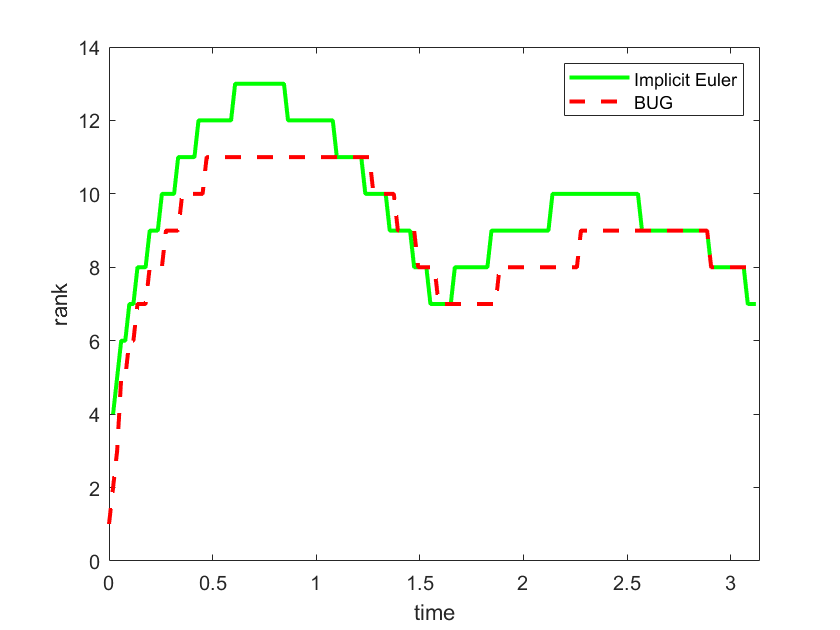
\includegraphics[width=0.75\linewidth]{rank-time.png}
        \caption{XXX}
    \end{figure}
\end{frame}

\begin{frame}{Columns}
    \begin{columns}
        \column{0.6\textwidth}
        \begin{figure}
            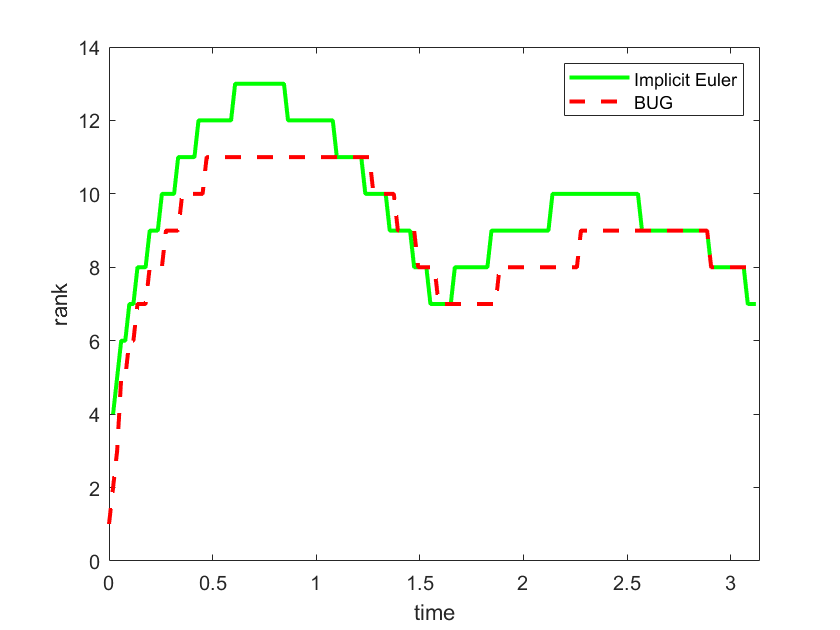
\includegraphics[width=\linewidth]{rank-time.png}
            \caption{XXX}
        \end{figure}
        \column{0.4\textwidth}
        This is column one with 0.4 text width.
    \end{columns}
\end{frame}

\begin{frame}{Figures}
    \begin{figure}[htbp]
        \centering
        \begin{subfigure}[b]{0.47\textwidth}
            \centering
            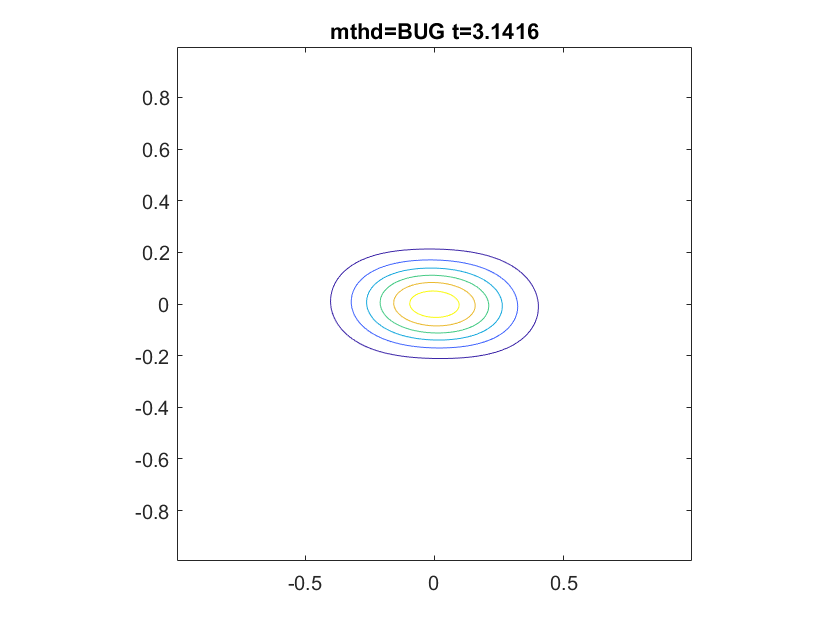
\includegraphics[width=\textwidth]{bug.png}
            \caption{XXX}
            \label{fig:subfig-a}
        \end{subfigure}
        \begin{subfigure}[b]{0.47\textwidth}
            \centering
            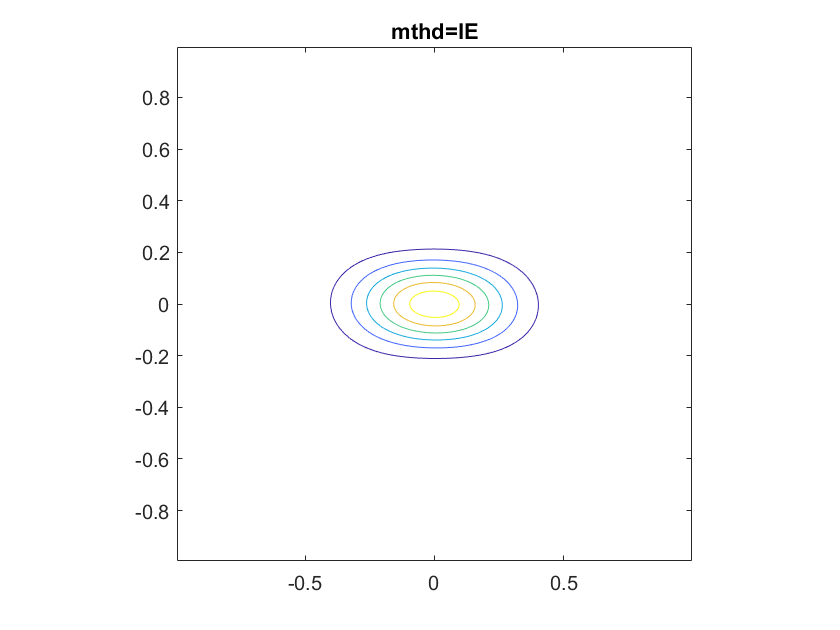
\includegraphics[width=\textwidth]{ie.png}
            \caption{XXX}
            \label{fig:subfig-b}
        \end{subfigure}
        \caption{XXX}
        \label{fig:example}
    \end{figure}
\end{frame}

\begin{frame}{Algorithm}
    \begin{algorithm}[H]
        \caption{Euclid's algorithm}
        \KwData{Two nonnegative integers $a$ and $b$}
        \KwResult{Their greatest common divisor $d = \gcd(a, b)$}
        \While{$b \neq 0$}{
            $r \leftarrow a \bmod b$\;
            $a \leftarrow b$\;
            $b \leftarrow r$\;
        }
        $d \leftarrow a$\;
    \end{algorithm}

\end{frame}

\begin{frame}[fragile]{Code}

    \begin{lstlisting}[language=c++]
#include <iostream>

int main() {
    std::cout << "Hello, world!" << std::endl;
    return 0;
}
\end{lstlisting}

    \begin{lstlisting}[language=python]
def greet(name):
    """
    greets the person passed in as a parameter.
    """
    print(f"Hello, {name}!")

greet("John")
\end{lstlisting}

\end{frame}


\section{Conclusion}

\begin{frame}{Conclusion}
    xxx xxx xxx xxx xxx xxx.
    xxx xxx xxx xxx xxx xxx.
    xxx xxx xxx xxx xxx xxx.
    xxx xxx xxx xxx xxx xxx.
\end{frame}

\begin{frame}{Future work}
    xxx.
\end{frame}


\end{document}
